\deu{\section{Stochastik}\index{Stochastik}}
\eng{\section{Stochastics}\index{Stochastics}}
\setcounter{aufgabenNummer}{1}
  \renewcommand{\kAufgabenBuchstabe}{S}

\subsection{\deu{Grundlagen}\eng{Basics}}

\kNiveauAufgabe{\deu{Mengenschreibweise von Ereignissen}\eng{Quantity notation of events}:
\deu{Eine Urne enthält 10 Kugeln mit den Zahlen 0 bis 9. Eine Kugel wird
gezogen.}
\eng{An urn contains 10 balls with the numbers 0 to 9. One single ball is drawn.}

\begin{enumerate}[label=\alph*)]
\item
\deu{
Geben Sie folgende Ereignisse in aufzählender Form an:

A: Die Kugel trägt als Zahl eine Primzahl.\\
B: Die Zahl auf der Kugel ist durch 5 teilbar.\\
C: Die Zahl auf der Kugel ist ungerade.\\
D: Die Zahl auf der Kugel ist > 8.\\
E: Die Zahl auf der Kugel ist > 20.\\
F: Die Zahl auf der Kugel ist eine Quadratzahl.\\
G: Sicheres Ereignis
}
\eng{
State the following events in enumerative form:

A: The number on the sphere is a prime number.\\
B: The number on the sphere is divisible by 5.\\
C: The number on the sphere is odd.\\
D: The number on the sphere is > 8.\\
E: The number on the sphere is > 20.\\
F: The number on the ball is a square number.\
G: Certain event
}%% end eng

\deu{
\item Zählen Sie alle Elementarereignisse auf.
\item Es wurde eine 7 gezogen. Welche der Ereignisse aus Teilaufgabe a) sind eingetroffen?
\item Welche Ereignispaare aus a) schliessen sich gegenseitig aus?
\item Beschreiben Sie die Gegenereignisse der unter a) aufgeführten
Ereignisse
}

\eng{
\item List all elementary events.
\item A 7 was drawn. Which of the events from subtask a) occurred?
\item Which pairs of events from a) are mutually exclusive?
\item Describe the counter-events of the events listed under a)
}
\end{enumerate}
}{%% Lösungen

a) $A = \{2, 3, 5, 7\}, B = \{0, 5\}, C = \{1, 3, 5, 7, 9\}, D = \{9\}, E = \{\}, F = \{0, 1, 4, 9\},\\ G = \{0, 1, 2, 3, 4, 5, 6, 7, 8, 9\}$

b) $\{0\}, \{1\}, \{2\}, \{3\}, \{4\}, \{5\}, \{6\}, \{7\}, \{8\}, \{9\}$

c) $A, C, G$

d) $A \cap D = \{\}, A \cap E = \{\}, A \cap F = \{\}, B \cap D = \{\}, B \cap  E = \{\},\\ C \cap E = \{\}, D \cap E = \{\}, E  \cap F = \{\}$


\kKommentar{dies ist eine Aufzählung, keine Beschreibung:}
e) $\overline{A} = \{0, 1, 4, 6, 8, 9\}, \overline{B} = \{1, 2, 3, 4, 6, 7, 8, 9\}, \overline{C} = \{0, 2, 4, 6, 8\}, \overline{D} = \{0, 1, 2, 3, 4, 5, 6, 7, 8\},\\
\overline{E} = \{0, 1, 2, 3, 4, 5, 6, 7, 8, 9\}, \overline{F} = \{2, 3, 5, 6, 7, 8\}, \overline{G} = \{\}$
}{8}


\kNiveauAufgabe{\deu{
Der Ergebnisraum $\Omega$ und seine Teilmengen (= Ereignisse):
Aus einer grossen Produktionsserie von Leuchtdioden werden nacheinander und zufällig drei
Stück entnommen (ohne Zurücklegen). Sie werden auf „defekt“ (d) bzw. „nicht defekt“ (n)
hin überprüft.}
\eng{The result space $\Omega$ and its subsets (= events):
From a large production series of light-emitting diodes (LED), three pieces are taken one after the other at random (without putting them back). They are checked for "defective" (d) or "not defective" (n).
}

\begin{enumerate}[label=\alph*)]
\deu{
\item  Geben Sie den Ergebnisraum $\Omega$ an.
\item  Geben Sie die Ereignisse A bis E als Teilmengen von $\Omega$ an:
A: Die zuerst entnommene Leuchtdiode ist defekt.\\
B: Die zuerst entnommene Leuchtdiode und nur diese ist defekt.\\
C: Alle entnommenen Leuchtdioden sind defekt.\\
D: Genau zwei entnommene Leuchtdioden sind defekt.\\
E: Mindestens zwei der entnommenen Leuchtdioden sind in Ordnung.\\
}
\eng{\item Specify the result space $\Omega$.
\item Specify the events A to E as subsets of $\Omega$:

A: The first light-emitting diode removed is defective.\\
B: The first light-emitting diode removed and only this one is defective.\\
C: All removed LEDs are defective.\\
D: Exactly two removed LEDs are defective.\\
E: At least two of the removed LEDs are OK.\\
}
\end{enumerate}
}{%% Lösungen
a) $$ \Omega = \{ddd, ddn, dnd, dnn, ndd, ndn, nnd, nnn\}$$

b) $A=\{ddd, ddn, dnd, dnn\}, B = \{dnn\}, C = \{ddd\}, D = \{ddn, dnd, ndd\},\\
E = \{dnn, ndn, nnd, nnn\}$
}{8}

\kNiveauAufgabe{
\deu{Wird beim Würfeln mit 2 gewöhnlichen Spielwürfeln Augensumme 7 (Ereignis A) oder Augensumme 8 (Ereignis B) häufiger auftreten?}
\eng{When rolling 2 ordinary dice, will the sum of 7 (event A) or the sum of 8 (event B) occur more frequently?}
}{%% Lösungen
\deu{Wahrscheinlichkeit für Augensumme 7 oder 8 mit zwei Würfeln}\eng{Probability of a sum of 7 or 8 with two dice}:\\

A: Augensumme 7: $A = \{$\epsdice{1}\epsdice{6}, \epsdice{2}\epsdice{5}, \epsdice{3}\epsdice{4}, \epsdice{4}\epsdice{3}, \epsdice{5}\epsdice{2}, \epsdice{6}\epsdice{1}$\}$
B: Augensumme 8: $B = \{\epsdice{2}\epsdice{6}, \epsdice{3}\epsdice{5}, \epsdice{4}\epsdice{4}, \epsdice{5}\epsdice{3}, \epsdice{6}\epsdice{2}\}$

$P(A) = \frac6{36}=\frac16, P(B) = \frac5{36}$

\deu{Die Summe 7 tritt häufiger auf als die Summe 8.}\eng{"The sum 7 occurs more frequently than the sum 8.}
}{8}


\subsection{\deu{Kombinatorik}\eng{Combinatorics}}\index{\deu{Kombinatorik}\eng{Combinatorics}}

\kNiveauAufgabe{\deu{Ein Bauer will zwei Kühe, drei Schweine und vier Legehennen von einem Viehhändler, der
sieben Kühe, fünf Schweine und 10 Legehennen zur Auswahl anbietet, kaufen. Auf wie viele
Arten kann der Bauer wählen?}
\eng{A farmer wants to buy two cows, three pigs and four laying hens from a livestock dealer who offers a choice of seven cows, five pigs and 10 laying hens. In how many ways can the farmer choose?}
}{%% Lösungen
$m={7\choose 2} \cdot{} {5\choose 3} \cdot{} {10\choose 4} = 44\,100$
}{8}

\kNiveauAufgabe{\deu{Zehn Lernende stehen in einer Reihe in der Mensa. Auf wie viele Arten kann die Reihe gebildet
werden?}\eng{Ten students stand in a row in the canteen. In how many ways can the row be formed?}
}{%% Lösungen
$$m=10! = 3\,628\,800$$
}{8}

\kNiveauAufgabe{\deu{An einer Party mit zwanzig Gästen stösst jeder Gast
mit jedem an. Wie oft erklingen die Gläser?}
\eng{At a party with twenty guests, every guest toasts
with everyone. How often do the glasses clink?}
}{%% Lösungen
$$m={20 \choose 2} = 190$$
}{8}

\kNiveauAufgabe{\deu{Wie viele Personen nehmen an einer Party teil,
wenn im ganzen 406-mal Gläser klingen (und jede Person mit jeder
andern angestossen hat)?}
\eng{How many people attend a party if glasses are clinked 406 times in total glasses clink (and each person has clinked glasses with every other person)?}
}{%% Lösungen
$$ {n\choose 2} = 406 \Longrightarrow x=29 $$
}{8}

\kNiveauAufgabe{
\deu{Ein Schüler will in den Sommerferien seine Schulbücher – ein Englischbuch, drei Deutschbücher, zwei Französischbücher und vier Mathematikbücher (alle Bücher sind verschieden!)
– ordnen. Sie sollen auf ein Regal gestellt werden, wobei Bücher des gleichen Fachgebietes
nebeneinander stehen sollen. Wie viele verschiedene Gruppierungsmöglichkeiten der Bücher
gibt es?}
\eng{During the summer vacation, a pupil wants to bring order into his
school books - one English book, three German books, two French books and four math books (all books are different!).
They are to be placed on a shelf, with books from the same subject stand next to each other.
In how many different ways can the books be grouped?
}
}{%% Lösungen
 $$m = (1! \cdot{} 3! \cdot{} 2!  \cdot{} 4!) \cdot{} (4!) = 6912$$
}{8}

\kNiveauAufgabe{\deu{Vier Personen steigen in ein Zugsabteil. Der Zug
fährt mit diesen vier Personen los und hält anschliessend noch an
sechs weiteren Haltestellen.}
\eng{Four people board a train compartment. The train departs with these four
people and then stops at six more stops.}
\begin{enumerate}[label=\alph*)]
\item \deu{Wie viele verschiedene Möglichkeiten haben die vier Personen, um den Zug zu verlassen
(es dürfen auch mehrere Personen gleichzeitig den Zug verlassen)?}
\eng{How many different ways do the four people have to get off the train

(several people can leave the train at the same time)?}
\item \deu{Wie viele Möglichkeiten gibt es, wenn jede Person an einer
andern Station aussteigt?}
\eng{How many possibilities are there if each «passenger» gets off at a
get off at a different station?}
\end{enumerate}
}{%% Lösungen
a) $6^4 = 1296$

b) $6\cdot{}5\cdot{}4\cdot{}3 = 360$
}{8}

\kNiveauAufgabe{\deu{Die Buchstaben aus dem Wort MISSISSIPPI werden durcheinandergemischt und zufällig
wieder zusammengesetzt. Wieviele verschiedene Buchstabenfolgen mit und ohne Bedeutung
können dabei entstehen?}
\eng{The letters from the word MISSISSIPPI are mixed up and are then randomly reassembled.
How many different sequences of letters with and without meaning can
result from this procedure?}
}{%% Lösungen
$$m=\frac{11!}{2!\cdot{} 4! \cdot{} 4!} = 34\,650$$
}{8}


\subsection{\deu{Wahrscheinlichkeit}\eng{Probability calculation}}
\kNiveauAufgabe{
\textbf{\deu{Arbeiten mit dem Gegenereignis}\eng{Working with the counter-event}}:
\deu{In einer Urne befinden sich 4 rote und 3 schwarze Kugeln, sowie 1 grüne Kugel. Es wird zwei
Mal hintereinander eine Kugel mit Zurücklegen gezogen. Bestimmen Sie die Wahrscheinlichkeit des Ereignisses A: „Mindestens eine rote Kugel ist dabei“. Suchen Sie zuerst das
Gegenereignis von A. Resultat in Bruchform.}
\eng{There are 4 red and 3 black balls and 1 green ball in an urn. A
ball is drawn twice in succession and put back. Determine the
probability of event A: "There is at least one red ball". First look
for the event of A. Write the result in fractional form.}
}{%% Lösungen
$P(\overline{A}) = \frac48\cdot{}\frac48 = \frac14, P(A) =
1-P(\overline{A}) = \frac34$
}{8}


\kNiveauAufgabe{\deu{Man wirft einen roten und einen grünen Würfel. Mit
welcher Wahrscheinlichkeit?}\eng{Roll one red and one green die. With
what probability}
\begin{enumerate}[label=\alph*)]
\item
\deu{wirft man einen Pasch (= 2 gleiche Werte)?}
\eng{is it a double (two similar values)?}
\item
\deu{ist die Augensumme gleich 5?}
\eng{is the sum equal to 5?}
\item
\deu{zeigt der grüne Würfel einen Punkt mehr als der rote?}
\eng{does the green die show one point more than the red die?}
\item
\deu{wirft man weder 3 noch 5?}
\eng{does it show neither 3 nor 5?}
\end{enumerate}
}{%% Lösungen
\begin{enumerate}[label=\alph*)]
\item $P=\frac16$
\item $P=\frac19$
\item $P=\frac5{36}$
\item $P=\frac49$
\end{enumerate}

}{8}

\kNiveauAufgabe{\deu{Für das einmalige Werfen eines verfälschten Spielwürfels
gilt diese Wahrscheinlichkeitstabelle:}
\eng{For the one-time roll of a falsified die this probability table applies:}

\renewcommand{\arraystretch}{1.8}
\begin{tabular}{|c|c|c|c|c|c|c|}\hline
\deu{Augenzahl}\eng{Points} $X=i$ &1 &2 &3 &4 &5 &6 \\\hline
$P(X=i)$   & $\frac15$ & $\frac16$ & $\frac2{15}$ & $\frac2{15}$ &
$\frac16$ & ?\\\hline
 \end{tabular}
\renewcommand{\arraystretch}{1}
 \deu{
 Berechnen Sie die Wahrscheinlichkeiten folgender Ereignisse:

A: keine gerade Augenzahl\\
B: Augenzahl grösser als 4\\
C: Gegenereignis von A.
}
\eng{Calculate the probabilities of the following events:


A: no even number\\
B: Number greater than 4\\
C: opposite event of A.}
}{%% Lösungen
$P(X=6) = 1-\frac15-\frac16-\frac2{15}-\frac2{15}-\frac16 = \frac15$

$P(A) = \frac12$

$P(B) = \frac{11}{30}$

$P(C) = \frac12$
}{8}

\kNiveauAufgabe{\deu{Zwei Münzen werden gleichzeitig geworfen. Man schaut,
ob Kopf oder Zahl fällt.}
\eng{Two coins are tossed at the same time. You look to see
whether heads or tails falls.}

\begin{enumerate}[label=\alph*)]
 \item \deu{Geben Sie die Ergebnismenge $\Omega$ an.}\eng{Specify the result set $\Omega$.}
 \item \deu{Geben Sie zu jedem Elementarereignis die zugehörige Wahrscheinlichkeit an.}\eng{Specify the associated probability for each elementary event.}
 \item \deu{Die Zufallsvariable $X$ sei „Anzahl Kopf“ im Wurf von 2 Münzen. Berechnen Sie die
   Wahrscheinlichkeiten für 0-mal Kopf, 1-mal Kopf und 2-mal Kopf.}
   \eng{Let the random variable $X$ be "number of heads" in the toss of 2 coins. Calculate the probabilities for 0 times heads, 1 time heads and 2 times heads.}
\end{enumerate}
   }{%% Lösungen
\begin{enumerate}[label=\alph*)]
\item $\Omega = \{kk, kz, zk, zz\}$
\item $P(kk) = P (kz) = P (zk) = P (zz) = \frac14$
\item $P(X=2)=\frac14, P(X=1)=\frac12, P(X=0)=\frac14$
\end{enumerate}
}{8}

\kNiveauAufgabe{\deu{Eine Münze wird drei Mal hintereinander geworfen. Wie gross ist die Wahrscheinlichkeit, dass
drei gleichartige Seiten oben liegen (drei Mal Kopf oder drei MalZahl)?}
\eng{A coin is tossed three times in succession. What is the probability that three identical sides come up (three times heads or three times tails)?}
}{%% Lösungen


 $P(kkk) = \left(\frac12\right)^3 = \frac18$

$P(zzz)= P(kkk) = \frac18$

\eng{hence}\deu{somit}: $P=P(kkk) + P(zzz) = \frac14$
}{8}

\kNiveauAufgabe{\deu{Ein Glücksrad hat 8 gleich grosse Sektoren mit den Nummern 1, 2, 1, 2, 3, 2, 1, 2.
Nach Stillstand des Rades zeigt der oberhalb des Rades fix montierte Pfeil auf einen Sektor
mit Nummer.}
\eng{A wheel of fortune has 8 equally sized sectors with the numbers 1, 2, 1, 2, 3, 2, 1, 2.
After the wheel has come to a standstill, the fixed arrow above the
wheel points to a sector with a number.}

\begin{enumerate}[label=\alph*)]
\deu{
\item Das Rad wird einmal gedreht. Mit welcher Wahrscheinlichkeit erscheint 2?
\item Das Rad wird zweimal gedreht. Mit welcher Wahrscheinlichkeit sind beide Ziffern gleich?
\item Das Rad wird fünfmal gedreht. Mit welcher Wahrscheinlichkeit ist die Ziffernfolge:
1 - 2 - 3 - 2 - 1?
}%% end deu

\eng{
\item The wheel is turned once. With what probability does 2 appear?

\item
The wheel is turned twice. What is the probability that both digits are the same?

\item
The wheel is turned five times. With what probability is the sequence of digits:
1 - 2 - 3 - 2 - 1?
} %% end eng

\end{enumerate}
}{%% Lösungen

a) $P(\{2\}) = \frac12$

b) $P(\{2-2; 1-1; 3-3\}) = \frac{13}{32}$

c) $P(\{12321\}) = \frac9{2048}$
}{8}



\kNiveauAufgabe{\deu{Eine Klasse besteht aus 10 Schülerinnen und 14
Schülern. Durch das Los werden 5 Personen
dieser Klasse ausgewählt. Wie gross ist die Wahrscheinlichkeit, dass}

\eng{A class consists of 10 female and 14 male
pupils. By drawing lots, 5 people are selected
of this class are selected by lot. What is the probability that}


\begin{enumerate}[label=\alph*)]
\item
\deu{alle fünf Personen Schülerinnen sind}\eng{all five people are female}?
\item
\deu{alle fünf Personen Schülerinnen sind}\eng{all five people are male}?
\item
\deu{unter den 5 Personen Schülerinnen und Schüler vorkommen}\eng{female and male pupils are among the five people}?

\end{enumerate}
}{%% Lösungen

\deu{Siehe auch Lotto Modell}\eng{see also: lottery-model}

a) $P=\frac{3}{506}$

b) $P={13}{276}$

c) $P = \frac{125}{132}$

}{8}

\kNiveauAufgabe{\deu{Aus Ihrer Klasse werden zufällig 3 Personen ausgewählt. Wie gross ist die Wahrscheinlichkeit,
dass ihre Geburtsmonate alle verschieden sind, wenn man annimmt, dass die Geburtsmonate
in der Klasse zufällig „verteilt“ sind?}

\eng{3 people are chosen at random from your class. What is the probability
that their months of birth are all different, assuming that the months
of birth are «randomly» distributed in the class?}
}{%% Lösungen

$P = \frac{12}{12} \cdot{} \frac{11}{12} \cdot{}  \frac{10}{12} = \frac{55}{72} \approx 76.4\%$

}{8}

\kNiveauAufgabe{\deu{In einem Gefäss befinden sich 5 rote, 5 blaue und
5 gelbe Kugeln. Es werden drei Kugeln aufs Mal gezogen. Wie gross ist
die Wahrscheinlichkeit, dass}
\eng{There are 5 red, 5 blue and 5 yellow balls in a container. Three balls are drawn at once. What is the probability that}
\begin{enumerate}[label=\alph*)]
\item
\deu{nur blaue Kugeln gezogen werden?}
\eng{only blue balls are drawn?}
\item
\deu{keine gelben Kugeln gezogen werden?}
\eng{only yellow balls are drawn?}
\end{enumerate}
}{%% Lösungen

a) $P = \frac5{15} \cdot{} \frac4{14} \cdot{} \frac3{13} = \frac2{91} \approx  2.20\%$

b) $P = \frac{10}{15} \cdot{} \frac9{14} \cdot{} \frac8{13} = \frac{24}{91} \approx  26.4\%$
}{8}


\kNiveauAufgabe{\deu{Ein Kasten enthält 2 schwarze, 2 rote und 6 grüne
Kugeln. Es werden nacheinander 3 Kugeln gezogen. Bestimmen Sie die
Wahrscheinlichkeit, drei verschiedene Farben zu erhalten, wenn}
\eng{A box contains 2 black, 2 red and 6 green balls. Three balls are drawn one after the other. Determine the probability of getting three different colors if}
\begin{enumerate}[label=\alph*)]
\item
\deu{ohne Zurücklegen gezogen wird.}
\eng{the balls are drawn \textbf{without} putting them back.}
\item
\deu{mit Zurücklegen gezogen wird.}
\eng{the balls are drawn \textbf{with} putting them back.}
\end{enumerate}
}{%% Lösungen


a) $P = 3! \cdot{} \frac2{10} \cdot{} \frac29 \cdot{} \frac68 = \frac15$

b) $P = 3! \cdot{} \frac2{10} \cdot{} \frac2{10} \cdot{} \frac6{10} = \frac{18}{125}$

}{8}

\kNiveauAufgabe{\deu{Ein normaler Spielwürfel wird sechs Mal geworfen. Mit welcher Wahrscheinlichkeit treten
sechs verschiedene Augenzahlen auf?}
\eng{A normal die is thrown six times. What is the probability of six different numbers occurring?}

\deu{(Ergebnis in \% auf 2 Stellen nach dem Komma gerundet.)}
\eng{(Result in \% rounded to 2 decimal places).}
}{%% Lösungen

$\frac5{324} \approx 1.54\%$
}{8}




\kNiveauAufgabe{\deu{An einem Chilbistand können ein oder mehrere Spieler
eine Anzahl Bälle kaufen und damit 
auf eine Scheibe werfen. Gewonnen hat jeweils der Spieler, der die
Scheibe als erster trifft.

Zwei Spieler, nennen wir sie A und B, kaufen je zwei Bälle, die sie einzeln und abwechselnd
(A zuerst) werfen. A und B sind nicht gleich geschickt in diesem Spiel: A trifft jeweils mit der
Wahrscheinlichkeit $\frac16$, B nur mit Wahrscheinlichkeit
$\frac1{10}$.  Wie gross ist die Wahrscheinlichkeit,
}

\eng{At a boot on a church festival, one or more players can buy a
number of balls and throw them at a target. The winner is the player
who hits the target first.

Two players, let's call them A and B, each buy two balls, which they
throw individually and alternately (A first). A and B are not equally
skilled in this game: 

A hits each with probability $\frac16$, B only with probability $\frac1{10}$.

What is the probability
}


\begin{enumerate}[label=\alph*)]
\item
\deu{dass die Scheibe bei allen vier Würfen nicht getroffen wird?}
\eng{ that the target will not be hit on all four throws?}
\item
\deu{dass Spieler A gewinnt, d.h. die Scheibe als erster trifft?}
\eng{that player A will win, i.e. be the first to hit the target?}
\end{enumerate}
}{%% Lösungen

a) $\frac9{16}$

b) $\frac7{24}$ 

}{8}

\kNiveauAufgabe{\deu{An einem Chilbistand können ein oder mehrere Spieler
eine Anzahl Bälle kaufen und damit auf eine Scheibe werfen. Gewonnen hat jeweils der Spieler, der die Scheibe als erster trifft.
Drei Spieler, nennen wir sie A, B und C, kaufen je zwei Bälle, die sie
einzeln und abwechselnd (Reihenfolge ABCABC) auf die Scheibe
werfen. A, B und C sind nicht gleich geschickt in 
diesem Spiel: B trifft jeweils mit der Wahrscheinlichkeit $\frac15$
und C nur mit Wahrscheinlichkeit $\frac1{12}$
.
Die Wahrscheinlichkeit, dass A schliesslich gewinnt (d.h. in seinem
ersten oder zweiten Wurf die Scheibe trifft), beträgt 0.25. Wie gross ist die Trefferwahrscheinlichkeit von A, d.\,h.
die Wahrscheinlichkeit dafür, dass A die Scheibe in jeweils einem Wurf
trifft? Resultat in \%
auf 2 Dezimalen gerundet.}
\eng{At a festival one or more players can buy a number of balls and
throw them at a target.
The winner is the player who hits the target first.

Three players, let's call them A, B and C, each buy two balls, which
they throw in turns at the tagert in the order ABCABC.

A, B and C are not equally skilled in this game in this game:

B hits the target with probability $\frac15$
and C only with probability $\frac1{12}$
The probability that A will ultimately win (i.e. in his first or second throw
first or second throw) is 0.25.

What is the probability of A hitting the target, i.\,e.
in one throw)?

Result in \% rounded to 2 decimals.}%% end english
}{%% Lösungen

$0 = -\frac{11}{15}p^2 + \frac{26}{15}p -\frac14 \Longrightarrow  P
= \frac{26-\sqrt{511}}{22} \approx 15.4\%$

\eng{the second solution is impossible}\deu{die zweite Lösung ist unmöglich}
}{8}


\subsubsection{\deu{Hypergeometrische Verteilung (Lotto-Modell)}%
\eng{Hypergeometric distribution (lottery-model)}}


\kNiveauAufgabe{
\deu{Beim Schweizer Zahlenlotto\footnote{Ein Swiss Lotto Tipp besteht aus 6 Zahlen (aus 42 Zahlen) sowie aus einer Glückszahl zwischen 1 und 6. Ein
Gewinn wird erzielt, wenn mindestens 3 Gewinnzahlen der Zahlenreihe 1 bis 42 richtig getippt werden. Wer alle
6 Zahlen zusammen mit der Glückszahl richtig voraussagt, knackt den Jackpot.} sind 6 Zahlen aus 42 (ohne
Wiederholung) zu wählen. Zudem muss eine Zusatzzahl zwischen 1 und 6
getippt werden.}
\eng{In the Swiss Lotto\footnote{A Swiss Lotto entry consists of 6 numbers (out of 42 numbers) and a lucky number between 1 and 6. A win is achieved if at least 3 winning numbers from the series 1 to 42 are guessed correctly. If someone correctly predicts all 6 numbers along with the lucky number, they hit the jackpot.}, 6 numbers out of 42 (without repetition) are to be chosen. Additionally, a bonus number between 1 and 6 must be guessed.}

\begin{enumerate}[label=\alph*)]
\item
\deu{Wie viele Auswahlmöglichkeiten gibt es für die 6 Zahlen aus 42?}
\eng{How many options are there for choosing 6 numbers out of 42?}

\item
\deu{Wie gross ist demnach die Wahrscheinlichkeit für einen
Lottosechser ohne Berücksichtigung der Zusatzzahl?}
\eng{What is the probability, therefore, of hitting the jackpot without considering the bonus number?}

\item
\deu{Wie gross ist die Wahrscheinlichkeit, genau 3 Richtige, jedoch eine falsche Zusatzzahl zu haben?}
\eng{What is the probability of having exactly 3 correct numbers but a wrong bonus number?}
\end{enumerate}
}{%% Lösungen

a) ${42 \choose 6} = 5\,245\,786$

\vspace{1mm}

b) $P = \frac1{5\,245\,786} \approx 1.906\cdot{}10^{-5}\%$

\vspace{1mm}

c) $P = \frac{{6\choose 3} \cdot{} {36\choose 3}}{{42 \choose
6}}\cdot{} \frac56 \approx 2.26849\%$
}{8}

\kNiveauAufgabe{\deu{Ein normales französisches Kartenspiel besteht aus 36 Karten. Davon tragen 9 Karten die
„Farbe“ Herz. Nun wird an einem Fest ein Glücksspiel gespielt: Je nach Geldeinsatz darf
man mehrere Karten ziehen (ohne Zurücklegen). Die Herzkarten gelten als Glückstreffer und
gewinnen einen kleinen Preis. Anna entnimmt dem Spiel 16 Karten. Wie gross ist die Wahrscheinlichkeit, dass unter den gezogenen Karten genau 5 Herzkarten, also Glückstreffer, dabei
sind? (Ergebnis in \% auf zwei Dezimalen gerundet.)}
\eng{A standard French deck of cards consists of 36 cards. Among them, 9 cards are of the 'hearts' suit. Now, at a festival, a game of chance is played: depending on the amount of money bet, one can draw several cards (without replacement). The heart cards are considered lucky hits and win a small prize. Anna draws 16 cards from the game. What is the probability that exactly 5 heart cards, i.e., lucky hits, are among the drawn cards? (Result rounded to two decimal places as a percentage.)}
}{%% Lösungen

$P= \frac{ {9 \choose 5} \cdot{} {27 \choose 11}}{{36 \choose 16}} \approx 22.48\%$

}{8}

\kNiveauAufgabe{\deu{In einer Schale befinden sich 30 Smarties, darunter 12 rote. David schnappt sich blind 10
Smarties. Wie gross ist die Wahrscheinlichkeit, dass er genau 6 rote
dabei hat?}
\eng{n a bowl, there are 30 Smarties, including 12 red ones. David blindly grabs 10 Smarties. What is the probability that he has exactly 6 red ones among them?}
}{%% Lösungen
$P= \frac{ {12 \choose 6} \cdot{} {18 \choose 4}}{{30 \choose 10}} \approx 0.012979\%$
}{8}

\kNiveauAufgabe{\deu{Wie gross ist die Wahrscheinlichkeit, im Euromillions
drei richtige Zahlen und zwei richtige Sterne zu haben? (Im Eurolotto müssen von 50 Zahlen fünf angekreuzt, sowie aus zwölf „Sternzahlen“
zwei ausgewählt werden.)}
\eng{What is the probability of having three correct numbers and two correct stars in EuroMillions? (In EuroMillions, out of 50 numbers, five must be selected, and two 'star numbers' must be chosen from twelve.)}
}{%% Lösungen

$P=
\frac{ {5 \choose 3} \cdot{} {45 \choose 2}}{{50 \choose 5}}
\cdot{}
\frac{ {2 \choose 2} \cdot{} {10 \choose 0}}{{12 \choose 2}}
\approx 0.0070796\%$

}{8}


\subsubsection{Bernoulli}

\kNiveauAufgabe{\deu{Man würfelt 4-mal hintereinander mit einem gewöhnlichen Spielwürfel. Wie gross ist die
Wahrscheinlichkeit, dass man genau 2 Sechser gewürfelt hat?}
\eng{You roll a standard six-sided die four times in a row. What is the probability of rolling exactly 2 sixes?}
}{%% Lösungen
$P \approx 11.574\%$
}{8}

\kNiveauAufgabe{\deu{In einem bestimmten Land rechnet man bei 53.5\% der Einzelgeburten mit einem Mädchen.
Eine Mutter hat fünf Kinder geboren (keine Mehrfachgeburten).}
\eng{In a certain country, 53.5\% of single births are expected to be girls. A mother has given birth to five children (no multiple births).}
\begin{enumerate}[label=\alph*)]
\item
\deu{Berechnen Sie die Wahrscheinlichkeit, dass sie 0, 1, . . . , 5
Mädchen hat.}
\eng{Calculate the probability that she has 0, 1, ..., 5 girls.}
\item
\deu{Veranschaulichen Sie diese Binomialverteilung in einem Histogramm: x-Achse: Anzahl
Mädchen in 5 Einzelgeburten (0, . . . , 5). y-Achse (Säulenhöhe):
Wahrscheinlichkeit (als Dezimalzahl oder in \%) für diese Anzahl.}

\eng{Illustrate this binomial distribution in a histogram: x-axis: Number of girls in 5 single births (0, ..., 5). y-axis (column height): Probability (as a decimal or in \%) for each number.}
\end{enumerate}

}{%% Lösungen

$P(0)\approx 2.17\%;
 P(1) \approx 12.5\%;
 P(2) \approx 28.8\%;
 P(3)\approx 33.1\%;
 P(4)\approx 19.0\%;\\
 P(5)\approx 4.38\%$

Histogram\deu{m}:

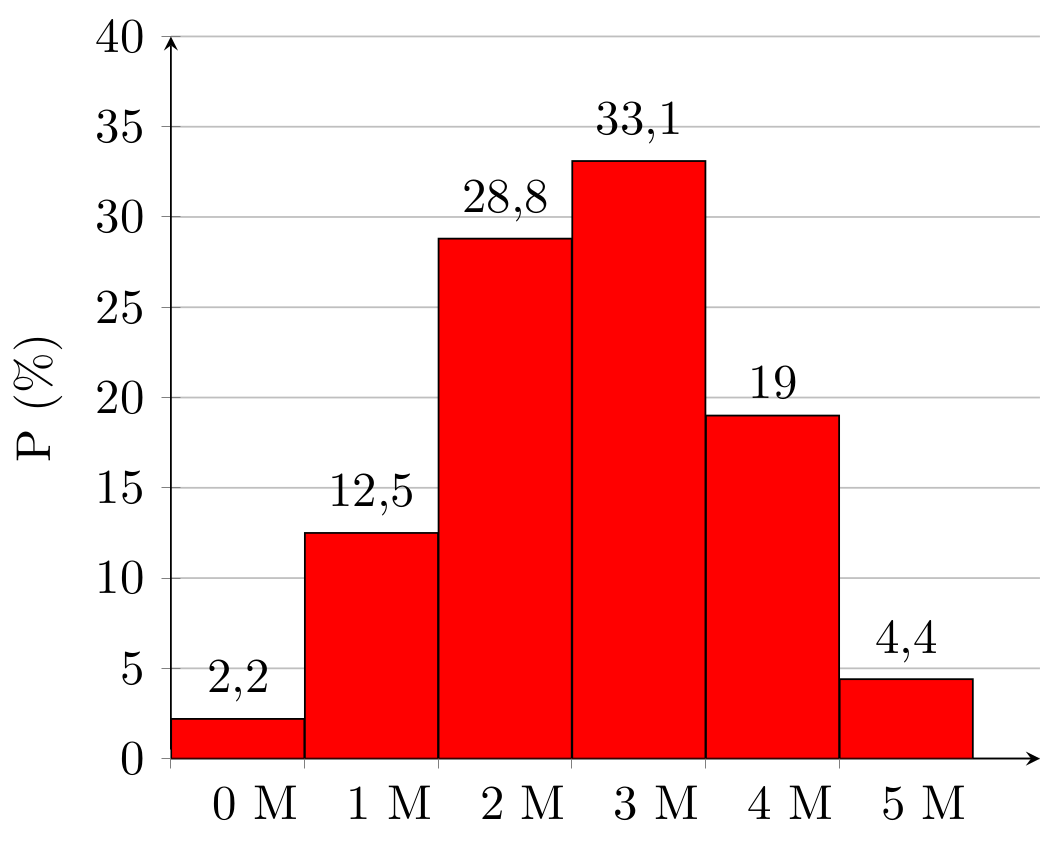
\includegraphics[width=80mm]{img/stoch/HistogrammGeburten.png}

}{8}

\kNiveauAufgabe{\deu{Nikolas ist ein guter Basketballspieler. Seine
Trefferquote beträgt beim Freiwurf 90\%.

a) Wie wahrscheinlich ist es, dass er bei genau 8 von 10 Freiwürfen trifft?\\
b) Wie gross ist die Wahrscheinlichkeit, dass er bei vier Freiwürfen mindestens einen Treffer
landet?}
\eng{ "Nikolas is a good basketball player. His free throw shooting
percentage is 90\%.

a) What is the probability that he makes exactly 8 out of 10 free
throws?

b) What is the probability that he scores at least one hit in four free throws?
}% end eng
}{%% Lösungen

a) $P\approx 19.37\%$

b) $P=99.99\%$

}{8}


\kNiveauAufgabe{
\begin{enumerate}[label=\alph*)]
\item \deu{Wie gross ist die Wahrscheinlichkeit, mit einem gerechten
Spielwürfel (Augenzahlen 1 bis 6) in 10 Würfen zwischen 3-mal und 7-mal eine Eins zu werfen?}
\eng{What is the probability, with a fair six-sided die (numbers 1 to 6), of rolling a one between 3 and 7 times in 10 rolls?}

\item \deu{Wie gross ist die Wahrscheinlichkeit, mit obigem Würfel in 10 Würfen entweder 0-mal
bis 2-mal oder 8-mal bis 10-mal eine Eins zu werfen?}
\eng{What is the probability, with the above die, of rolling a one
either 0 to 2 times or 8 to 10 times in 10 rolls?}

\item \deu{Erstellen Sie mit Hilfe des Taschenrechners eine
Wertetabelle für die Wahrscheinlichkeiten, in 10 Würfen 0-mal, 1-mal,
. . . , 10-mal eine Eins zu würfeln. Erstellen Sie mit 
diesen Daten ein Balkendiagramm.}

\eng{Using the calculator, create a value table for the probabilities
of rolling a one 0 times, 1 time, ..., 10 times in 10 rolls. Use this
data to create a bar-chart.}

\newcommand{\ppp}{\,\hspace{8mm}\,}%% Platz Platz Platz

\begin{tabular}{c|c|c|c|c|c|c|c|c|c|c|c}
 $k$  & 0 & 1 & 2 & 3 & 4 & 5 & 6 &7 & 8 & 9 & 10 \\\hline
 $P$  & \ppp  & \ppp  & \ppp  & \ppp  & \ppp  & \ppp  & \ppp  & \ppp &  \ppp & \ppp  &
\ppp \end{tabular} 

\end{enumerate}
}{%% Lösungen

a) $P\approx 6.946\%$

b) $P\approx 77.5246\%$

c)

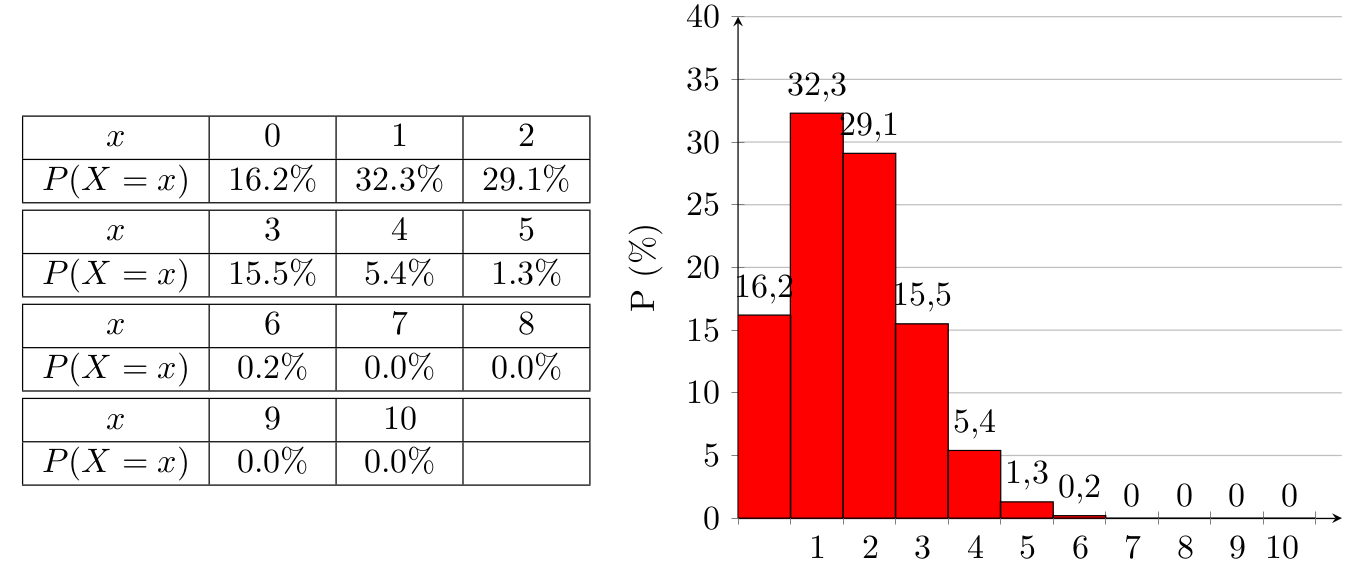
\includegraphics[width=150mm]{img/stoch/WuerfelBarChart.png}

}{8}




\subsubsection{\deu{Kontingenztafeln und bedingte Wahrscheinlichkeit}\eng{Contingency tables and conditional probability}}

\kNiveauAufgabe{\deu{Von einer seltenen Krankheit sind nur 0.5\% der Bevölkerung betroffen. Ein Test zeigt bei
Gesunden in 95\% der Fälle zu Recht ein negatives Resultat; in den
restlichen 5\% der gesunden  Fälle zeigt der Test
fälschlicherweise ein positives Ergebnis („false positive“). Bei Kranken zeigt der Test richtigerweise in 95\% der Fälle ein positives Resultat und in 5\% der Fälle fälschlicherweise ein
negatives Resultat (Nichterkennen der Krankheit).}

\eng{Only 0.5\% of the population is affected by a rare disease. A test correctly shows a negative result in 95\% of cases for healthy individuals; in the remaining 5\% of healthy cases, the test falsely indicates a positive result ('false positive'). For those with the disease, the test correctly shows a positive result in 95\% of cases and falsely indicates a negative result in 5\% of cases (failure to recognize the disease).}

\begin{enumerate}[label=\alph*)]
\item
\deu{Stellen Sie die Situation am Beispiel eines
Bevölkerungsquerschnitts von 100’000 Personen in einer Vierfeldertafel
dar (absolute Zahlen eintragen).}
\eng{Illustrate the situation using a 2x2 table with the example of a population cross-section of 100,000 people (enter absolute numbers).}


\renewcommand{\arraystretch}{2}
\begin{center}\begin{tabular}{|l|c|c|c|}\hline
                            & positiv\eng{e}  & negativ\eng{e}
                            & \,\,\,\,\,\,Total \,\,\,\,\, \\\hline
\deu{krank}\eng{disease}    &                 &                &      \\\hline
\deu{gesund}\eng{healthy}   &                 &                &      \\\hline
Total                       &                 &                &      \\\hline
 \end{tabular}\end{center}
\renewcommand{\arraystretch}{1}


\item
\deu{Wie viele (richtige und falsche) positive Testresultate sind
insgesamt zu erwarten?}
\eng{How many (true and false) positive test results are to be expected in total?}
\item
\deu{Ermitteln Sie den zu erwartenden prozentualen Anteil an „false positive“-Resultaten
gemessen an allen positiven Resultaten. Runden Sie auf eine Dezimale.}
\eng{Determine the expected percentage of 'false positive' results relative to all positive results. Round to two decimal places.}
\end{enumerate}
 
}{%% Lösungen

a)

\renewcommand{\arraystretch}{2}
\begin{tabular}{|l|r|r|r|}\hline
                            & positiv\eng{e}  & negativ\eng{e} &   Total  \\\hline
\deu{krank}\eng{disease}    &    475          &   25           & 500      \\\hline
\deu{gesund}\eng{healthy}   &   4\,975        &   94\,525      & 99\,500  \\\hline
Total                       &   5\,450        &   94\,550      & 100\,000 \\\hline
 \end{tabular}
\renewcommand{\arraystretch}{1}

b) ca 5450 Test positiv\eng{e}

c) $\frac{4975}{5450} \approx 91.28\%$

}{8}

\newcommand{\kHorizPlatz}{\hspace{25mm}}

\kNiveauAufgabe{\deu{Beim 1000-maligen Einschalten einer Anlage fällt
Bauteil A 70-mal und Bauteil B 100-mal aus. 22-mal fallen dabei beide
Bauteile gleichzeitig aus. Stellen Sie eine Vierfeldertafel auf und
geben Sie die folgenden relativen Häufigkeiten an: }
\eng{During the 1000 activations of a system, component A fails 70 times, and component B fails 100 times. Both components fail simultaneously 22 times. Set up a 2x2 table and provide the following relative frequencies:}

\begin{enumerate}[label=\alph*)]
\item
\deu{Mindestens eines der beiden Bauteile fällt aus.}
\eng{At least one of the two components fails.}
\item
\deu{Genau eines der beiden Bauteile fällt aus.}
\eng{Exactly one of the two components fails.}
\end{enumerate}

\renewcommand{\arraystretch}{2}
\begin{tabular}{|c|c|c|c|}\hline
 \kHorizPlatz{}       &   \kHorizPlatz{}       &  \kHorizPlatz{}     & \kHorizPlatz{}  \\\hline
         &          &         &      \\\hline
         &         &         &      \\\hline
         &         &         &      \\\hline
 \end{tabular}
\renewcommand{\arraystretch}{1}
 

}{%% Lösungen

\renewcommand{\arraystretch}{2}
\begin{tabular}{|c|c|c|c|}\hline
 \kHorizPlatz{}              &   A \eng{fails}\deu{fällt aus}  & A OK  & \kHorizPlatz{}  \\\hline
 B \eng{fails}\deu{fällt aus}& 22         &  78       & 100     \\\hline
 B OK                        & 48        &  852       &   900   \\\hline
                             & 70        & 930        & 1000     \\\hline
 \end{tabular}
\renewcommand{\arraystretch}{1}


a) $|E| = 22+48+78 = 148 \Longrightarrow P=\frac{148}{1000} = 14.8\%$

b) $|E| = 48 + 78 = 126 \Longrightarrow P=\frac{126}{1000} = 12.6\%$
}{8}



\kNiveauAufgabe{
\deu{Eine Schafherde besteht aus 240 Tieren. Das Fell von 75\% der Schafe ist einfarbig, der Rest
ist mehrfarbig. Ein Drittel der Tiere ist jünger als zweijährig. 50
Schafe sind mehrfarbig und nicht jünger als zwei Jahre alt. Beantworten Sie mit Hilfe einer Vierfeldertafel folgende Frage: Wie viele
Schafe sind einfarbig und jünger als zweijährig?}
\eng{A flock of sheep consists of 240 animals. The fleece of 75\% of the sheep is solid-colored, and the rest is multicolored. One-third of the animals are younger than two years. 50 sheep are multicolored and not younger than two years old. Answer the following question using a 2x2 table: How many sheep are solid-colored and younger than two years?}

\renewcommand{\arraystretch}{2}
\begin{tabular}{|c|c|c|c|}\hline
 \kHorizPlatz{}       &   \kHorizPlatz{}       &  \kHorizPlatz{}     & \kHorizPlatz{}  \\\hline
         &          &         &      \\\hline
         &         &         &      \\\hline
         &         &         &      \\\hline
 \end{tabular}
\renewcommand{\arraystretch}{1}
 

}{%% Lösungen

\renewcommand{\arraystretch}{2}
\begin{tabular}{|c|c|c|c|}\hline
 \kHorizPlatz{}       &  \deu{einfarbig}\eng{solid-colored}  & \deu{mehrfarbig}\eng{multi-colored}     & \kHorizPlatz{}  \\\hline
  \deu{jung}\eng{young}       &   70       & 10        &   80   \\\hline
  \deu{nicht jung}\eng{not young}       &  110       &   50      & 160     \\\hline
         &   180      &     60    & 240     \\\hline
 \end{tabular}
\renewcommand{\arraystretch}{1}

\deu{70 Tiere sind einfarbig und jünger als zweijährig.}
\eng{70 animals are solid-colored and younger than two years.}

}{8}


\kNiveauAufgabe{
\deu{Der Betreiber einer Ostseefähre hat unter seinen Passagieren eine Umfrage durchgeführt. 10\%
der Passagiere reisten 1. Klasse. 65 der Passagiere der 2. Klasse waren mit den Leistungen des
Unternehmens zufrieden. Allerdings waren 70\% der Reisenden der 1. Klasse unzufrieden.
Betrachtet werden folgende Ereignisse:


$E$: Eine befragte Person reiste 1. Klasse. $\overline{E}$ ist das Gegenereignis.

$Z$: Eine befragte Person war zufrieden. $\overline{Z}$ ist das Gegenereignis.}

\eng{
The operator of a Baltic Sea ferry conducted a survey among its passengers. 10\% of the passengers traveled first class. 65 passengers in the second class were satisfied with the company's services. However, 70\% of the first-class travelers were dissatisfied. The following events are considered:

$E$: A surveyed person traveled first class. $\overline{E}$ is the complementary event.

$Z$: A surveyed person was satisfied. $\overline{Z}$ is the complementary event.
}

\begin{enumerate}[label=\alph*)]
\item
\deu{Erstellen Sie eine vollständig ausgefüllte Vierfeldertafel (E, E, Z, Z).}
\eng{Create a fully filled two-way table (E, E, Z, Z).}
\item
\deu{Als der Geschäftsleitung die Zufriedenheitszahlen der 1. Klasse mitgeteilt werden, ist
diese enttäuscht und meint, die Zufriedenheitszahlen aller Passagiere vom Vorjahr von
77\% nicht gesteigert zu haben. Beurteilen Sie diese Aussage.}
\eng{When the management is informed about the satisfaction numbers of the first class, they are disappointed and state that they have not exceeded the satisfaction numbers of all passengers from the previous year, which were 77\%. Evaluate this statement.}

\end{enumerate}

\renewcommand{\arraystretch}{2}
\begin{tabular}{|c|c|c|c|}\hline
 \kHorizPlatz{}       &   \kHorizPlatz{}       &  \kHorizPlatz{}     & \kHorizPlatz{}  \\\hline
         &          &         &      \\\hline
         &         &         &      \\\hline
         &         &         &      \\\hline
 \end{tabular}
\renewcommand{\arraystretch}{1}
 

}{%% Lösungen

a)

\renewcommand{\arraystretch}{2}
\begin{tabular}{|c|c|c|c|}\hline
 \kHorizPlatz{}    &   $E$    &  $\overline{E}$   & Total \\\hline
    $Z$            &   3\%    &  75\%             &  78\%   \\\hline
$\overline{Z}$     &   7\%    &  15\%             & 22\%     \\\hline
 Total             &   10\%   &   90\%            & 100\%     \\\hline
 \end{tabular}
\renewcommand{\arraystretch}{1}

b)

\deu{Das Total der Zufriedenen (78\%) ist leicht gestiegen.}

\eng{The total of satisfied individuals (78\%) has slightly increased.}

}{8}



\subsection{\deu{Statistisches Schließen}\eng{Statistical reasoning}}

\kNiveauAufgabe{\deu{Lukas bringt zu einem Würfelspiel seinen eigenen Spielwürfel mit. Es entsteht der Verdacht
Lukas' Würfel zeige überdurchschnittlich viele Sechsen an. Man beschliesst, einen Versuch
durchzuführen: Es wird 30-mal gewürfelt. Es wird vereinbart: Wenn 10-mal oder öfter eine
Sechs erscheint, erklären wir „Lukas“ Würfel als gefälscht. Lukas sagt: „Selbst wenn der Test
zehn oder mehr Sechsen ergibt, heisst das keineswegs, dass mein Würfel gefälscht ist; das
Resultat kann auch bei einem unverfälschten Würfel eintreten“. Wie
gross ist diese Wahrscheinlichkeit, dass in 30 Würfen ein gerechter
Würfel 10 oder mehr Sechsen anzeigt?}
\eng{Lukas brings his own dice to a dice game. The suspicion arises that Lukas' dice show an above-average number of sixes. It is decided to carry out an experiment: The dice are rolled 30 times. It is agreed: If a six appears 10 times or more, we declare "Lukas'" dice to be fake. Luke says: «Even if the test produces ten or more sixes, that doesn't mean that my die is fake; the result can also occur with a genuine die». What is the probability that a fair die will show 10 or more sixes in 30 throws?}
}{%% Lösungensum

$P(X\ge 10) = \sum_{x=10}^{30}{{30\choose x}} \cdot{} \left(\frac16\right)^x \cdot{} \left(\frac56\right)^{30-x}  = 1 - \sum_{i=0}^9 \approx 1.97\%$ 

\deu{
Die Wahrscheinlichkeit, dass ein nicht gezinkter Würfel bei 30 Würfen mehr
als 9 Sechsen anzeigt ist demnach ca. 2\%.

Mit ca. 2\% ist das Resultat den meisten wohl noch nicht eindeutig genug.
}
\eng{The probability that an unbiased die shows more than 9 sixes in
30 rolls is therefore approximately 2\%.

With about 2\%, the result may not be clear enough for most people.}%% end eng
}{8}

\newpage
